\subsubsection{subfunction-oeSetCrisisHandler}

\label{RE-use-case-oeSetCrisisHandler}


goal is to declare himself as been the handler of a crisis having the specified id.


\begin{usecase}
  \addheading{Use-Case Description}
  \addsingletwocolumnrow{Name}{oeSetCrisisHandler}
  \addsingletwocolumnrow{Scope}{system}
  \addsingletwocolumnrow{Level}{subfunction}
  
\addrowheading{Parameters}
\addnumberedsinglerow{AdtCrisisID: dtCrisisID}{}

\addrowheading{Primary actor(s)}
\addnumberedsinglerow{}{\msrcode{actCoordinator[active]}}


\addrowheading{Secondary actor(s)}
\addnumberedsinglerow{}{\msrcode{actCoordinator[passive]}}
\addnumberedsinglerow{}{\msrcode{actComCompany[passive, multiple]}}

\addrowheading{Goal(s) description}
\addsinglerow{goal is to declare himself as been the handler of a crisis having the specified id.
}

\addrowheading{Protocol condition(s)}
\addnumberedsinglerow{}{
}

\addrowheading{Pre-condition(s)}
\addnumberedsinglerow{}{
}

\addrowheading{Main post-condition(s)}
\addnumberedsinglerow{}{
}

\addrowheading{Additional Information}
\addsinglerow{
none
}

\end{usecase} 

Figure \ref{fig:lu.uni.lassy.excalibur.examples.icrash-RE-UCD-uc-oeSetCrisisHandler}
shows the use case diagram for the oeSetCrisisHandler subfunction use case

\begin{figure}[htbp]
\begin{center}

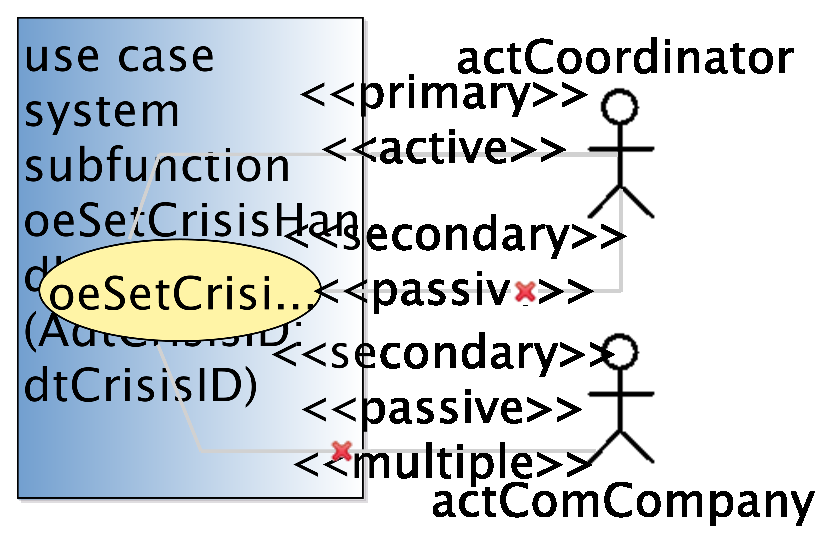
\includegraphics[
angle=0
,scale=0.75
]{./images-report-gen/usecase-model/subfunction/uc-oeSetCrisisHandler.eps}
\end{center}
\caption[lu.uni.lassy.excalibur.examples.icrash Use Case Diagram: uc-oeSetCrisisHandler]{oeSetCrisisHandler subfunction use case
}
\label{fig:lu.uni.lassy.excalibur.examples.icrash-RE-UCD-uc-oeSetCrisisHandler}
\end{figure}
\vspace{0.5cm}
